% chap4.tex (Evaluation)
\newpage
\thispagestyle{empty}
\mbox{}


\chapter{Evaluation}\label{EVAL-CHAP}
Many test scenarios have been executed during the setup of the testbed, variety of issues were found in the setup process (see Chapter \ref{IMPL-CHAP}). Therefore, approaches were changed and the code has been modified based on the outcome. In this chapter, I describe only those scenarios which gave the best results considering the resource limitation of the emulation testbed. In Section \ref{sec:tbcfg}, I give the details about the basic configuration of the testbed. In Section \ref{sec:expscn}, I talk about the experiment scenario I executed for evaluation and analysis. In Section \ref{sec:poct}, I describe the proof of concept test scenario and their results.. In Section \ref{sec:rgra}, I talk about report generation and the analysis of the execution results. Finally in Section \ref{sec:cws}, I compare the results of both simulation and emulation environment.


\section{Testbed Configuration}\label{sec:tbcfg}
Emulation scenario executed in both Mininet and MaxiNet platforms. Execution scenario of Mininet platform is executed in one single machine with 4 core Intel i5-3320M CPU running at 2.60GHz having 8GB RAM. The hardware details of MaxiNet platform is specified in section \ref{sec:infra}.

\subsection{Topology}
I used mesh topology for execution of all the evaluation scenarios in Mininet and used both mesh and ring topology for MaxiNet scenarios. While setting up the network, the model specified in \cite{7343600} was used and its overview as explained in that paper is described here. All the nodes are placed on a regular grid with a mean inter-node distance of $\bar{s} = 1000m$ and they are shifted in both $x$ and $y$ directions by normally distributed random variables with zero mean and a standard deviation of $\frac{\bar{s}}{8}$. In the mesh topology, a link between two nodes is created if the distance between them is less or equal to $1.5 \times \bar{s}$. A maximum link bandwidth of 500Mb is set for mesh topology link. The model for ring topology used here is a back-haul modeled similarly to the metro ring \cite{tbiermann}. In the ring topology, the ring center and the radius is calculated based on $\bar{s}$ and $\sqrt{number\ of\ nodes}$. Links are created between the nodes which are on the circumference of the ring with link bandwidth of 750Mb and other nodes are connected to its nearest neighbor node in the ring with the link of 500Mb bandwidth. Out of all nodes, some nodes are capable of running CAs; a probability value of 0.6 is used to decide if a node is a potential candidate for a CA or not. A maximum processing capacity of 40 GFLOPS is set for all nodes capable of being CA.

It is important to know that while creating the emulation network, those limitations are not introduced. That means all the Mininet/MaxiNet nodes (switches, hosts) are sharing the complete processing capacity of the hardware it is running on. Similarly, no bandwidth limitation is introduced on the link created between the Mininet/MaxiNet nodes. FlexFCAPF knows which node has how much processing capacity and which link has how much bandwidth; when the algorithm sees an LCA does not have enough processing capacity to satisfy a DFG, it will not assign any DFG to that LCA. Therefore, it is not necessary to emulate those limitations in the emulation network. Moreover, for introducing bandwidth capacity limitation, some traffic control objects need to be created and for limiting CPU processing capacity, process group need to be created for each node. I did not see any benefits of doing that and furthermore, it will load the testbed by eating some processing capacity of the hardware.
 
\subsection{Traffic Model}
Researchers usually use the Poisson process for traffic generation of circuit-switched data as well as packet data. The number of incoming packets or calls per time unit follows the Poisson distribution. The length or the duration of each phone call is typically modeled as an exponential distribution. Emulation also uses similar traffic generation model mentioned in this paper \cite{7343600} while simulation uses a non-stationary Poisson process with $\lambda = |V| \times loadlevel(t)$ and the thinning method \cite{Law:1999:SMA:554952} for DFG generation. A daily load level curve (see Figure \ref{fig:24loadlevel}) is prepared based on the cellular data traffic characteristics explained in \cite{Zhang:2012:UCC:2342468.2342472}. In emulation, the same model for traffic generation is used with a modified $\lambda = |V| \times loadlevel(t, scaling)$. Load level factor $scaling$ is added to set the scaling of the load level; this is done to control load level for different scenario and due to the hardware resource limitation in the emulation environment. The duration of the DFG is set by an exponential variable with parameter $0.02$ which means the expected average duration is 50 seconds and that an approximated number of DFGs in the network at any time $t$ is $50 \times |V| \times loadlevel(t, scaling)$. The execution scenario is divided into two sections based on flow types. One is the generic \cite{7343600} scenario and another is CoMP \cite{MArasha} scenario. Attributes specified in Table \ref {tab:gendfgtype} for generic scenario and in Table \ref {tab:compdfgtype} for CoMP scenario are used while generating DFGs.

\begin{table}[h!]
	\centering
	\caption{Generic data flow group types \cite{7343600}}
	\label{tab:gendfgtype}
	\begin{tabular}{c | c | c | c}
		\hline
		Type & Probability & $b_{flow}$ & $l_{flow}$\\
		\hline
		voice & 0.5 & 500 Kbits/s & 5 ms\\
		video & 0.4 & 1 to 4 Mbits/s & 10 ms\\
		data & 0.1 & 1 to 20 Mbits/s & 50 ms\\
		\hline
	\end{tabular}
\end{table}

\begin{table}[h!]
	\centering
	\caption{CoMP data flow group types \cite{MArasha}}
	\label{tab:compdfgtype}
	\begin{tabular}{c | c | c | c}
		\hline
		Type & Probability & $b_{flow}$ & $l_{flow}$\\
		\hline
		JP & 0.5 & 15 to 20 Mbits/s & 1 to 5 ms\\
		JSJB & 0.5 & 5 to 10 Mbits/s & 1 to 5 ms\\
		\hline
	\end{tabular}
\end{table}

\section{Experiment Scenario}\label{sec:expscn}
All scenarios are executed for a total of 2 hours real-time, and a 24 hours traffic pattern is emulated in 1-hour real-time duration. There are two reasons for reducing the execution time to 2 hours. First, there is an issue with running Ryu SDN controller for a long period. I observed whenever there are many flows in the network, i.e., the OVS has to deal with many traffic flows at a time, the OVS restarts. Now when the OVS instance restarts it tries to reconnect to the SDN controller. The SDN controller allows the client connection but gives a message saying multiple connections for same the DPID. This means the SDN controller still holds the previous connection information of the same switch in its memory. And due to this, I see many socket connections with CLOSE\_WAIT state in the system and its number keep increasing. After the number of open files reached a limit, the SDN controller can not open a new connection due to resource unavailability. This causes the SDN controller to die. Ideally, this reconnection from OVS should be handled in the SDN controller. While it would help to know why the OVS instance restarts when there are many traffic flow, I did not analyze it because it is out of the scope of this thesis. Therefore, I reduced the runtime to 2 hours so that I don't get an SDN controller failure. Also, by reducing the execution time, I could run multiple executions on the same day, i.e., I could emulate 2 days traffic pattern in just 2 hours (see Figure \ref{fig:24loadlevel}).

I want to clarify one important aspect of the emulation execution here. I used two terminologies frequently, i.e., emulation time and system time or real-time. Emulation time is basically the duration for which the execution will run and system time is the real time of the day. For example, I started an emulation execution at 3:00 PM real time for 2 hours duration so the execution will end at 5:00 PM. At the start, the emulation time is 0 and system time is 3:00 PM, and after 5 minutes of execution, the emulation time is 5 minutes (300 seconds) and system time is 3:05 PM and at the end of execution, the emulation time would be 2 hours and system time would be 5:00 PM. Emulation time increases by a value received by calling a random value generation (i.e., random.expovariate(lambdamax)) but system time will increase based on the system clock. In case the emulation time moves ahead of the system time, the execution will sleep for the time difference to be in sync with the emulation time (see Section \ref{sec:emuexec}). This way, emulation time can never go ahead of the system time and makes sure the emulation executes in real-time. There could be a scenario when the system time may move faster than the emulation time, in that case, I simply wait for the emulation time to catch up with the system time. This can happen when there is huge load on the system, which means, many DFG to process, traffic control objects to configure, and iperf instances and socat child processes to run. This means the system will take more time than the emulation time, and eventually the emulation time will stay far behind the system time. This is one main reason for introducing the load level scale to reduce the load in the emulation environment. Higher load level scale means more DFG in the system and it will take more time to process and the emulation time will never be able to catch it. The load level scale makes the execution design flexible if in the future I get a hardware with higher CPU power and memory; the load level scale can also be increased.

Table \ref{tab:evalscen} shows the list of scenarios I executed for analyzing FlexFCAPF in emulation environment. Other than that, I executed some proof of concept (POC) test scenarios and described it in section \ref{sec:poct}.
\begin{table}[h!]
	\centering
	\caption{Evaluation scenario}
	\label{tab:evalscen}
	\begin{tabular}{|c||c|c|c|c|c|}
	\hline
	\textbf{Scenario Id} & \textbf{Platform} & \textbf{Nodes} & \textbf{Topology} & \textbf{DFG Type} & \textbf{Scale}\\
	\hline
	1 & Mininet & 16 & mesh & generic & 0.40\\
	\hline
	2 & Mininet & 16 & mesh & CoMP & 0.05\\
	\hline
	\hline
	3 & MaxiNet & 36 & mesh & generic & 0.20\\
	\hline
	4 & MaxiNet & 36 & ring & generic & 0.20\\
	\hline
	5 & MaxiNet & 36 & mesh & CoMP & 0.02\\
	\hline
	6 & MaxiNet & 36 & ring & CoMP & 0.02\\
	\hline
	\end{tabular}
\end{table}

There are two scenarios executed in Mininet emulation, one for generic flow types and another for CoMP flow types. For generic flow type scenario, load scale of 0.40 is used and for CoMP the load level of 0.05 is used. Since the DFGs of CoMP flow types demand high processing power at the CA and high bandwidth in the link, the reduced load scale is used. Moreover, all the CoMP DFGs have multiple flows, which means to satisfy a CoMP DFG, the CA need to assign more processing power and the same goes for the link bandwidth. For example, if a DFG demands 5 FLOPS of processing power and 100Kb of link bandwidth and the DFG have 3 flows in it, to satisfy that DFG, the CA has to assign $5 \times3$ FLOPS processing power and the used link bandwidth in the network path in total would be $100\times3$ Kb. I also used only 16 nodes for both Mininet emulation, because Mininet has to run on a single machine and all the other applications (SDN controller, FlexFCAPF, the traffic generator etc.) are running on the same machine so I could not run with more nodes. In Mininet, only mesh topology is used because a ring topology with only 16 nodes would not be much different than a mesh topology.

There are four scenarios in MaxiNet emulation, two with mesh topology and two with a ring topology. For each topology, one is for generic flow type and another one for CoMP flow type. For all the MaxiNet scenarios, I used 36 nodes network. For the generic flow type, the load scale of 0.20 was used and for CoMP flow type, the load scale of 0.02 was used. Using these load level scales, I found all the DFG in the system are satisfied, except for scenario 1, only in some occasion I see some unsatisfied DFG in the system. There is no benefit of having more unsatisfied DFG is the system because that does not meet the emulation evaluation's purpose.

\section{Proof of Concept Testing}\label{sec:poct}
I executed some tests to verify the concepts which I introduced as part of the emulation, I describe them in this section.
\subsection{DFG Processing Test}
I explained how I implemented delay time in the interface in the host running as CA for DFG processing in the testbed in section \ref{sec:tmfg} and I have developed a small python script to test the DFG processing capability. This script establishes UDP connection to the LCA socat listener and send a packet and wait for it to come back. It measures the time difference between packet send time and packet receive time and save the time difference. While preparing the packet, the script adds the appropriate filter match pattern in the packet data field so that the right delay is applied in the LCA. The script continuously send 1,000 packet one after another and save the time difference.
\begin{figure}[tb]
	\begin{center}
		\resizebox{\textwidth}{!}
		{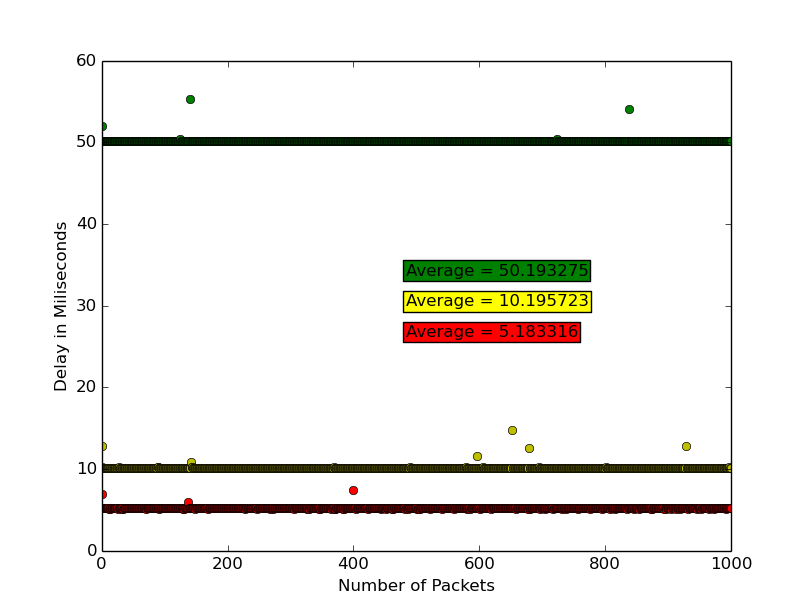
\includegraphics{delayplot-3-1-1000.png}}
		\caption{Delay for single flow.}
		\label{fig:delayplotsingle}
	\end{center}
\end{figure}

To test that script, I set up an emulation environment without dynamic DFG generation, configure the traffic control objects in the LCAs, and then execute that script from a node targeting its LCA. I ran the script for 5ms, 10ms, and 50ms delay. Figure \ref{fig:delayplotsingle} shows the time difference plotted for 5ms (red), 10ms (yellow), and 50ms (green) of delay for all 1,000 packets. I observed an average extra time of 200 microseconds taken for each packet and I assumed that this extra time includes sending the packet to the server, the latency between the client and server, processing at the server, receiving the packet at the client, and calculating and saving the time difference.
\begin{figure}[tb]
	\begin{center}
		\resizebox{\textwidth}{!}
		{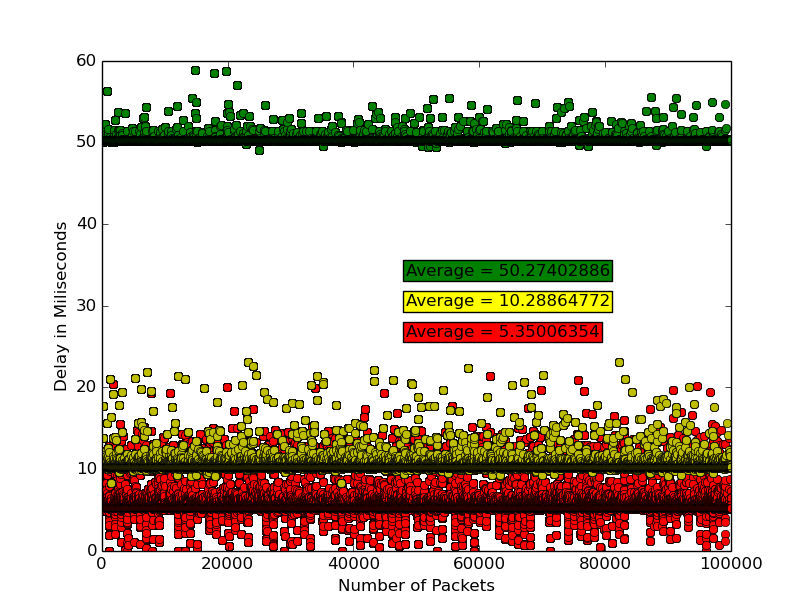
\includegraphics{delayplot-3-100-1000.png}}
		\caption{Delay for multiple flows.}
		\label{fig:delayplotmulti}
	\end{center}
\end{figure}

Similarly, I developed another small python script for testing packet loss and also to test the performance of the DFG processing capability when there is multiple parallel flow transmission happening. This script spawn 100 child processes executing the previous script. This means that in this case, there are 100 connections between a node and its LCA and each connection sends 1,000 packets one after another and save the time difference between sending and receiving of packets.

Same set up is used like the previous one to execute this multi-connection script. For most of the execution, the client could establish all 100 connections and receive returned packet for all the packets sent, which is why it could calculate the time difference for each packet. This also means there is no packet loss in the network. There are some occurrences where some clients could not establish the connection (3-4 out of 100); this might happen while the socat listener is busy serving another request. Figure \ref{fig:delayplotmulti} shows the time difference plotted for 5ms (red), 10ms (yellow), and 50ms (green) of delay for all $100\times1,000$ packets. In this case, I observed an average extra time of 300 microseconds taken for each packet.

I observed a similar pattern in both Mininet and MaxiNet platforms; here the given plot is generated in a MaxiNet platform where the source node and the LCA are running in the different MaxiNet worker.

\subsection{Traffic Generation Test}
I am using iperf to generate UDP traffic in the testbed and while starting iperf client instance, two parameters was passed, one for specifying data rate and one for the duration (see Section \ref{sec:tragen}). I saved the log for each iperf instance run and generated a report based on that log file for every evaluation scenario I executed.

\begin{figure}[tb]
	\begin{center}
		\resizebox{\textwidth}{!}
		{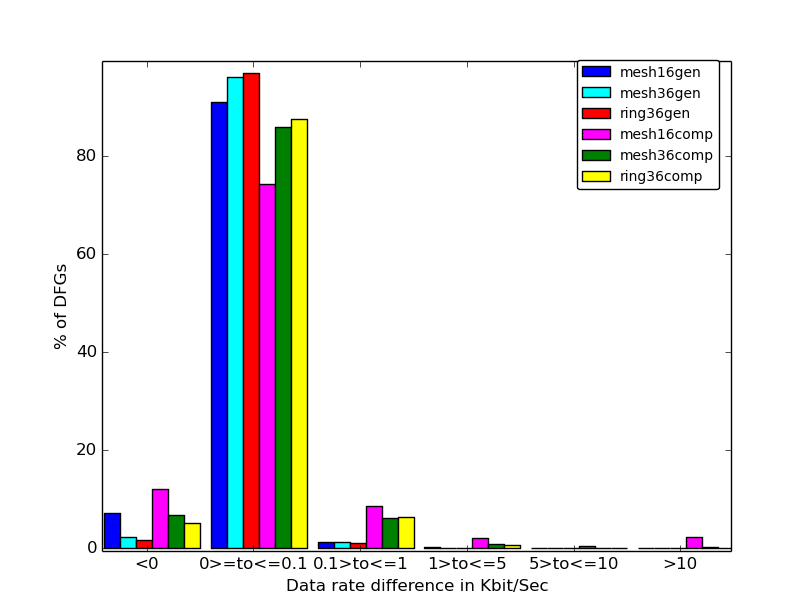
\includegraphics{bandwidthdiff.png}}
		\caption{Desired data rate vs generation data rate.}
		\label{fig:bandwidthdiff}
	\end{center}
\end{figure}

\begin{figure}[tb]
	\begin{center}
		\resizebox{\textwidth}{!}
		{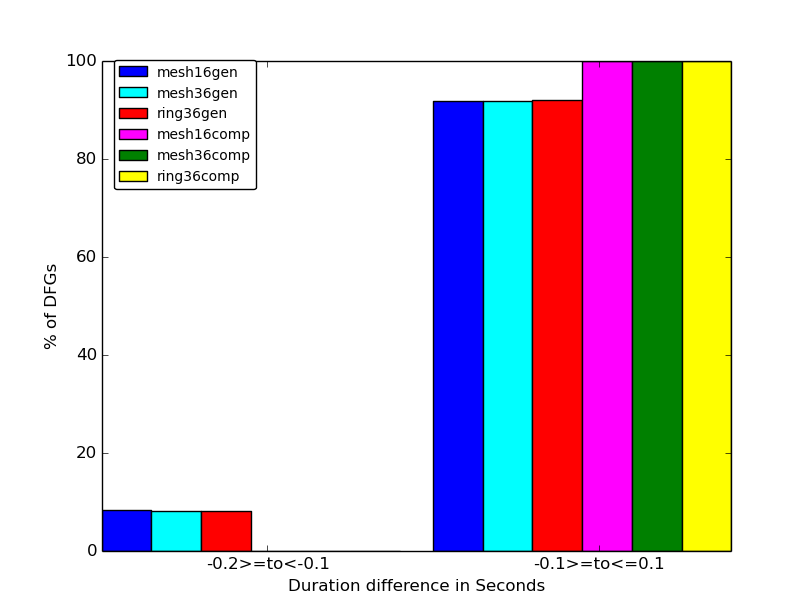
\includegraphics{timediff.png}}
		\caption{Expected duration vs generation duration.}
		\label{fig:timediff}
	\end{center}
\end{figure}

Figure \ref{fig:bandwidthdiff} shows the chart of expected data rate vs the actual data rate achieved while generating traffic. In Scenario 1 (blue) (see Table \ref{tab:evalscen}), the difference between desired data rate and generation data rate is 91\% of DFG between 0 to 0.1Kb/sec, 7\% less than 0Kb/sec (i.e., more data rate generated than expected), and 1\% greater than 0.1kb/sec. Iperf usually does not take the exact value for data rate or duration specified via command line but does some rounding of the specified value. For example, an iperf instance started with -b 9076381.59126 (data rate) and -t 45.26262756281 (duration), but iperf generated traffic of 9076386 bits/sec for 45.3 seconds. Another case, the iperf instance started with -b 9736626.21994 and -t 6.6471337635, but iperf generated traffic of 9736568bits/sec for 6.6 seconds. Thus, it is expected that iperf will sometimes round to a higher value and sometimes lower value. Similar data rate difference pattern to scenario 1 is observed in scenario 3 (cyan) and 4 (red). For scenario 2 (magenta), 5 (green), and 6 (yellow), the number of flow with a difference of 0.1 Kb/sec to 1Kb/sec is higher and the number of flows with the difference of less than 0Kb/sec also higher. These are CoMP scenarios and it demands higher data rate. This means iperf rounding may occur in higher range in both directions (negative or positive) if higher value passed with -b option while starting the iperf instance but none of the scenario show a huge difference between the desired rate and achieved rate. This proves that the data rate control of flow generation is working as expected in the testbed.

Figure \ref{fig:bandwidthdiff} shows the chart of expected duration of traffic generation vs actual duration for which actually the generation happened. In scenario 1 (blue) (see Table \ref{tab:evalscen}), for 92\% DFG the difference is in the range between -0.1 to 0.1 sec and 8\% DFG in the range of greater than -0.2 to less than -0.1 sec (a negative difference means traffic generation for more time than expected). A similar pattern is observed in scenario 3 (cyan) and 4 (red). For scenario 2 (magenta), 5 (green), and 6 (yellow), 100\% DFGs are in range of -0.1 to 0.1 sec difference. Even though for data rate, iperf round the passed value in both directions, i.e., either in lower or higher value, but usually iperf rounds the time parameter in higher value than it specified. This is the reason I observed for almost all the DFG; the difference between desired duration and generation duration is either 0 or negative. Though the rounding happens in ms range, there is not a single instance where the duration difference is very high. This proves that the duration control of flow generation is working as expected.

\subsection{Traffic Path Test}
FlexFCAPF decides the path for each DFG to follow, and based on the provided path, I added the forwarding entries in the underlying network elements. To verify whether the forwarding entries are correctly configured as per the path specified, I used \textit{Wireshark}. Figure \ref{fig:trafficpath} shows dump of UDP packet starting from host with IP 10.0.0.9 to destination host with IP 10.0.0.4. FlexFCAPF algorithm assigned the path to follow is: $s_8$ to $s_4$ to $s_3$; accordingly, the forwarding entries are added in the switches. Host 10.0.0.9 is connected to interface id 0 of $s_8$, $s_4$ is connected to the interface id 2 of $s_8$, $s_8$ is connected to interface id 11 of $s_4$, $s_3$ is connected to interface id 12 of $s_4$, $s_4$ is connected to interface id 13 of $s_3$ and host 10.0.0.4 is connected to interface id 7 of $s_3$.

\begin{figure}[tb]
	\begin{center}
		\resizebox{\textwidth}{!}
		{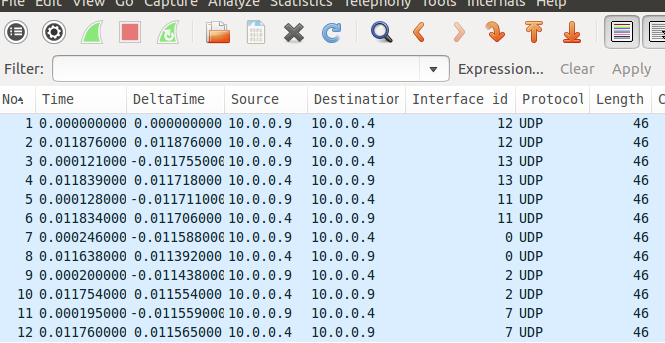
\includegraphics{h8toh3viah4.png}}
		\caption{Wireshark dump of a packet.}
		\label{fig:trafficpath}
	\end{center}
\end{figure}
In the Wireshark dump, we can see two packets passed through each of the interface, one with source IP 10.0.0.9 and destination IP 10.0.0.4, and another with source IP 10.0.0.4 and destination IP 10.0.0.9. This information proves two points: first the generated traffic follows exactly the path I configured and second, each packet goes to the destination (i.e., LCA) and LCA reply the same packet (same size of 46 Byte) back to the source. This is the kind of a DFG processing I wanted to implement in LCA.

\section{Reports Generation and Result Analysis}\label{sec:rgra}
I saved different dynamic statistics during execution of the scenarios specified in section \ref{sec:expscn} and based on those statistics, I generated some reports which I describe in this section.

As I already outlined in Section \ref{sec:expscn}, time difference ($t_d$) means emulation time ($t_e$) - system time passed from the start($t_s$). For example, I start an emulation at 3:00:00 PM for 2 hours (7,200 seconds); after some time, I got $t_e = 305$ and 3:05:00 PM is registered in the system clock time. This means the system clock moved 5 minutes (300 seconds) or equivalent to $t_s = 300$, so $t_d = t_e - t_s$ (i.e., $t_d=305-300=5$). Consider another situation, where I got $t_e=590$ and retrieved system clock time 3:10:00 PM. This means from the start the system time moved 10 minutes so $t_s=600$, and in this case $t_d=590-600=-10$. As I mentioned earlier, if the emulation time moved ahead of the system time (i.e., $t_d$ is positive), the emulation sleeps for the time difference and if emulation time is behind (i.e., $t_d$ is negative), then I assume emulation time will catch up with the system time.

Another terminology I used in this section is run-time ($t_r$). This is basically the length of real-time a process took to complete its task. I plotted two run-time for all the execution, one for algorithm run-time ($t_{ar}$) and another for reconfiguration run-time ($t_{rr}$). The $t_{rr}$ includes time spent on modifying routing path, configuring traffic control objects, and starting iperf instances needed after the execution of FelxFCAPF algorithm.

I collected all the time statistics before the emulation goes to sleep (if required) and all the plot I made in this section keeps emulation time ($t_e$) in the x-axis.

\subsection{Test Scenario 1}
This scenario was executed in Mininet platform with load level scale set to 0.40, mesh topology was used and the type of flow generated for the scenario is generic. Figure \ref{fig:ts1timediff} shows the plotting of $t_d$ against $t_e$. I observed both positive and negative $t_d$, which means occasionally $t_s$ is behind of $t_e$ or vice versa. A range of +1.34 to -1.23 seconds $t_d$ was observed. This is an expected behavior when there are many DFG added in the system which means more processing time is needed to configure traffic control objects and start iperf instances because of that $t_s$ moves ahead of $t_e$ and when few DFG is added in the system, $t_s$ is behind $t_e$ and the emulation would sleep for the $t_d$.

\begin{figure}[H]
	\begin{center}
		\subfloat[Emulation time vs time difference]{
			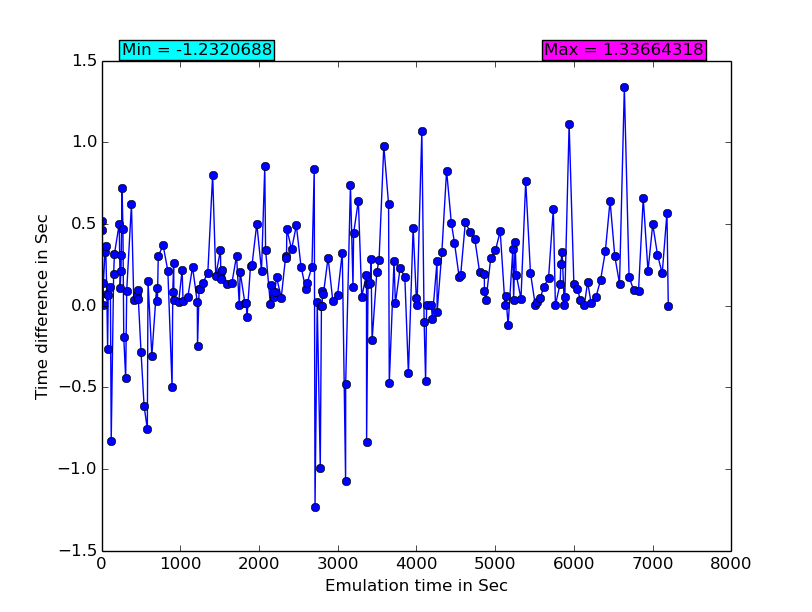
\includegraphics[width=0.48\textwidth]{16mesh40gentimediff.png}
			\label{fig:ts1timediff}
		}
		\subfloat[Emulation time vs runtime]{
			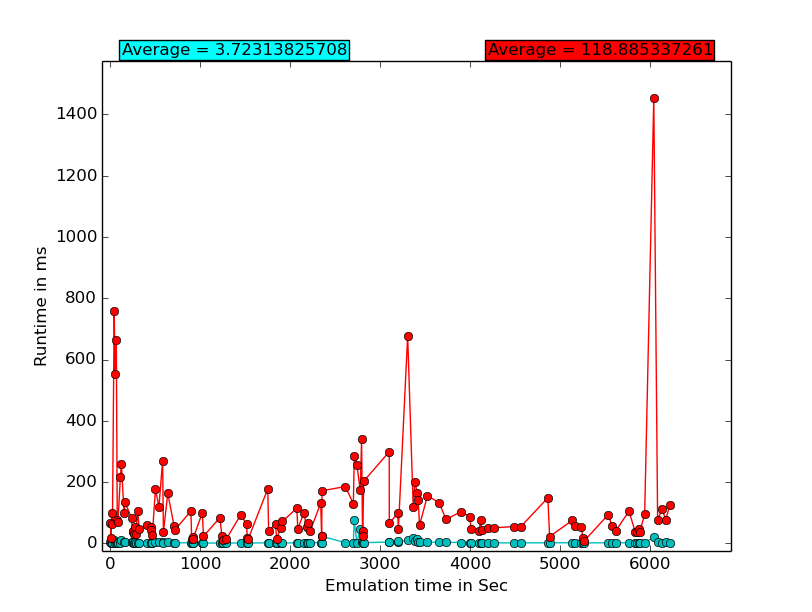
\includegraphics[width=0.48\textwidth]{16mesh40genruntime.png}
			\label{fig:ts1runtime}
		}
	\end{center}
\end{figure}

Figure \ref{fig:ts1runtime} has two statistics: the plotting of $t_{ar}$ against $t_e$ (cyan) and $t_{rr}$ against $t_e$ (red). Average $t_{ar}$ is around 3.72 ms whereas the average $t_{rr}$ is around 118.89 ms. Though the emulation for this scenario was executed for 7,200 seconds, the last algorithm execution was observed at 6,219 seconds, since there has been no more reassignment after this. There is few big spike of $t_{rr}$ seen, which means in that algorithm run, there are many DFG reassigned, which is why the system took more time to reset the routing entries, configure traffic control objects, and start iperf instances.

\subsection{Test Scenario 2}
This scenario was also executed in Mininet platform, the load level scale was set to 0.05, mesh topology was used and the type of flow generated for the scenario is CoMP. Figure \ref{fig:ts2timediff} shows the plotting of $t_d$ against $t_e$. Both positive and negative $t_d$ of +10.34 to -31.74 seconds is observed in this scenario. Here, $t_d$ has bigger range since it is a CoMP scenario; when there is heavy load the testbed has to start many iperf instances and configure many traffic control objects. This task takes time which is why more $t_s$ has passed while $t_e$ does not move much. In another case, while load level scale is low (0.05), then the emulation has to add very few DFG in the system because of that $t_e$ move ahead of the system time.

\begin{figure}[H]
	\begin{center}
		\subfloat[Emulation time vs time difference]{
			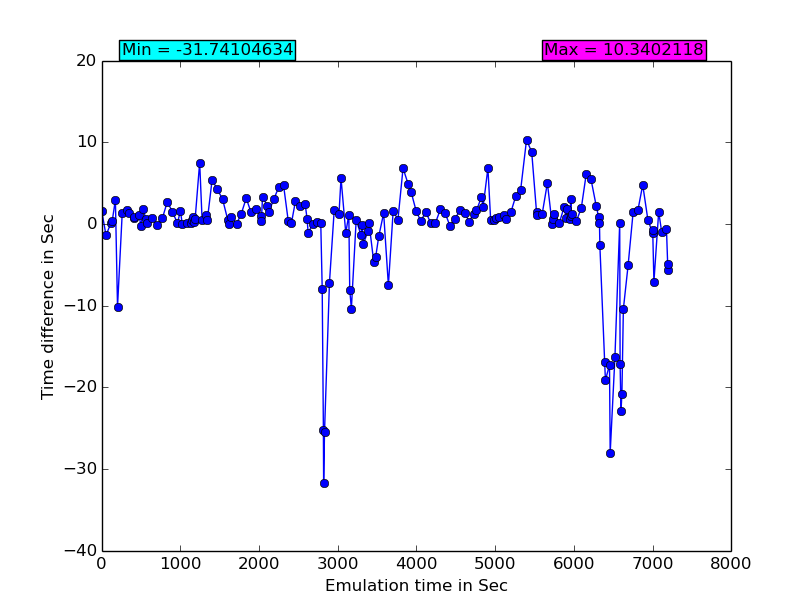
\includegraphics[width=0.48\textwidth]{16mesh05comptimediff.png}
			\label{fig:ts2timediff}
		}
		\subfloat[Emulation time vs runtime]{
			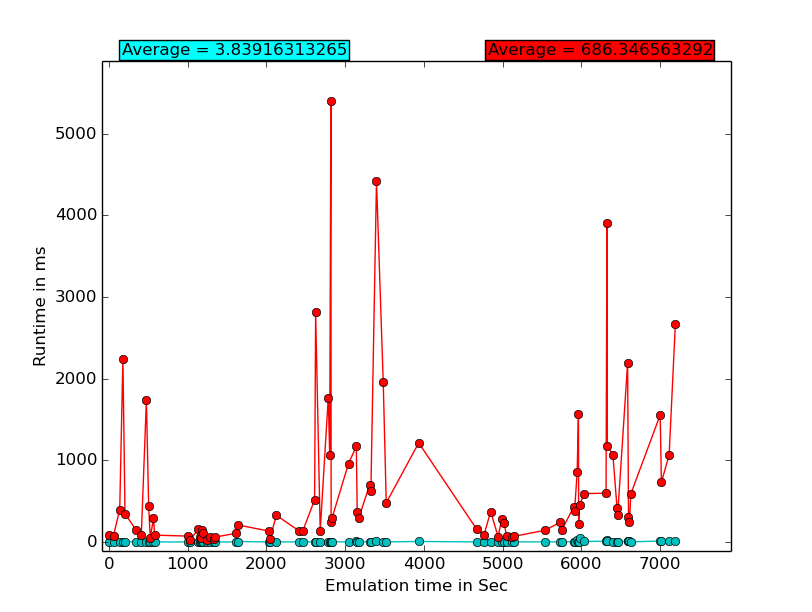
\includegraphics[width=0.48\textwidth]{16mesh05compruntime.png}
			\label{fig:ts2runtime}
		}
	\end{center}
\end{figure}

Similar to scenario 1, Figure \ref{fig:ts2runtime} has two statistics: the plotting of $t_{ar}$ against $t_e$ (cyan) and $t_{rr}$ against $t_e$ (red). Average $t_{ar}$ is around 3.83 ms and the average $t_{rr}$ is around 686.34 ms. The average $t_{rr}$ is higher because for CoMP flow type, usually numerous traffic control objects need to be added, and for a single DFG, multiple traffic flow generation has to be started. Similar to scenario 1, there are few big spikes of $t_{rr}$ seen, which means in that algorithm run, there were many DFGs reassigned. Compared to scenario 1, here I observed bigger gaps between the dots, which means less number of algorithm execution has happened.

\subsection{Test Scenario 3}
This scenario was executed in MaxiNet platform, the load level scale was set to 0.20, mesh topology was used, and the type of flow generated for the scenario is generic. Figure \ref{fig:ts3timediff} shows the plotting of $t_d$ against $t_e$. Both positive and negative $t_d$ of +0.89 to -0.73 seconds was observed in this scenario. Since load scale is medium and flow type is generic, a low range $t_d$ has been observed in this case.

\begin{figure}[H]
	\begin{center}
		\subfloat[Emulation time vs time difference]{
			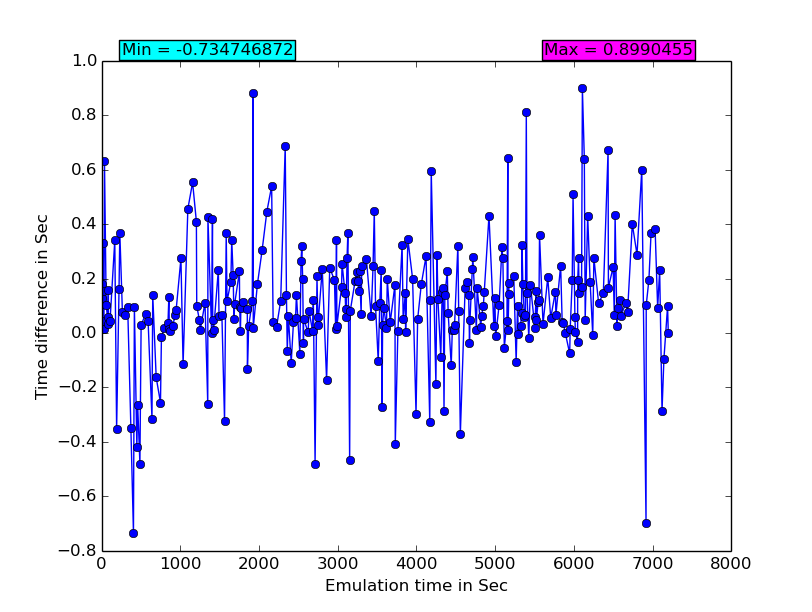
\includegraphics[width=0.48\textwidth]{36mesh20gentimediff.png}
			\label{fig:ts3timediff}
		}
		\subfloat[Emulation time vs runtime]{
			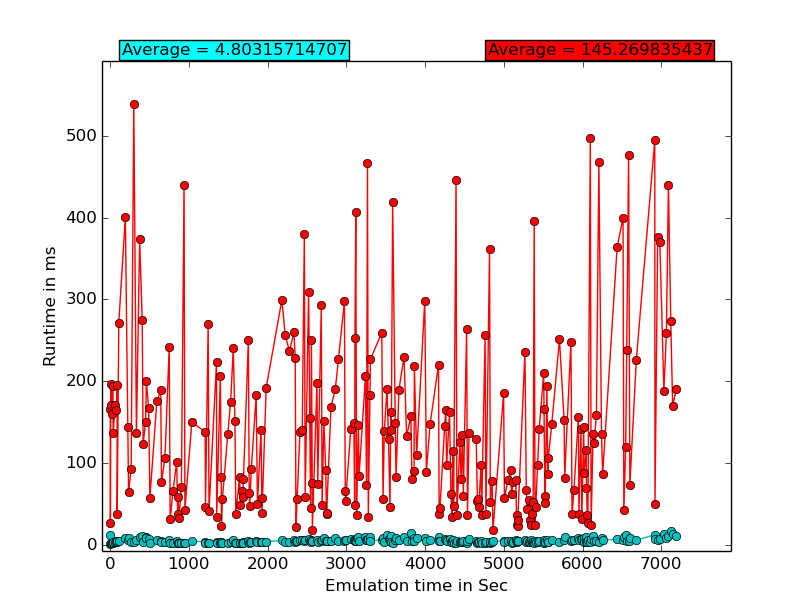
\includegraphics[width=0.48\textwidth]{36mesh20genruntime.png}
			\label{fig:ts3runtime}
		}
	\end{center}
\end{figure}

Similar to other scenarios Figure \ref{fig:ts3runtime} has two statistics: the plotting of $t_{ar}$ against $t_e$ is in cyan and $t_{rr}$ against $t_e$ is in red. Average $t_{ar}$ is around 4.08 ms and the average $t_{rr}$ is around 145.27 ms. The average $t_{rr}$ is low because for generic flow types, very few traffic control objects are needed to create since most DFG have similar processing delay. Like the other generic scenario, I also observed here fewer gaps between dots, which means the algorithm execution happened very frequently.

\subsection{Test Scenario 4}
This scenario was also executed in MaxiNet platform, the load level scale was set to 0.20, a ring topology was used and the type of flow generated for the scenario is generic. Figure \ref{fig:ts4timediff} shows the plotting of $t_d$ against $t_e$. Both positive and negative $t_d$ of +1.43 to -0.91 seconds was observed in this scenario. Similar to scenario 3, the load scale is medium and flow type is generic so a low range $t_d$ was observed in this case.

\begin{figure}[H]
	\begin{center}
		\subfloat[Emulation time vs time difference]{
			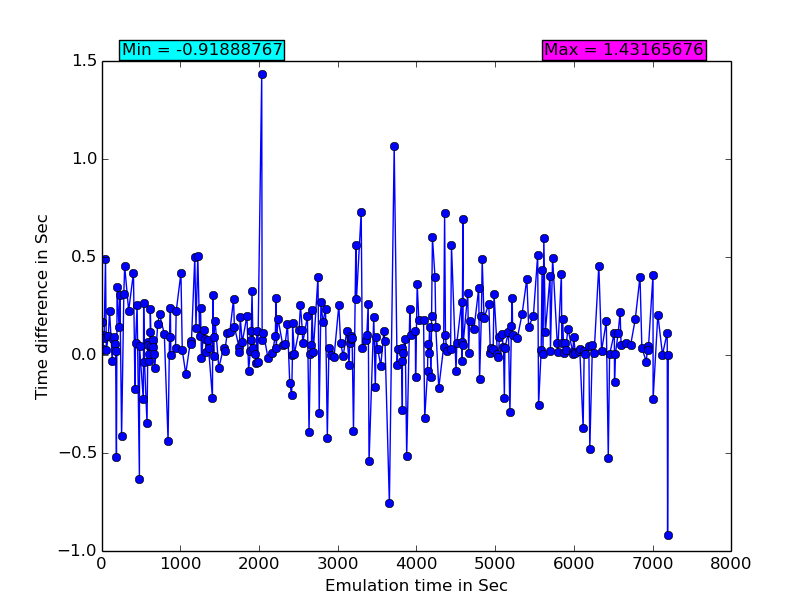
\includegraphics[width=0.48\textwidth]{36ring20gentimediff.png}
			\label{fig:ts4timediff}
		}
		\subfloat[Emulation time vs runtime]{
			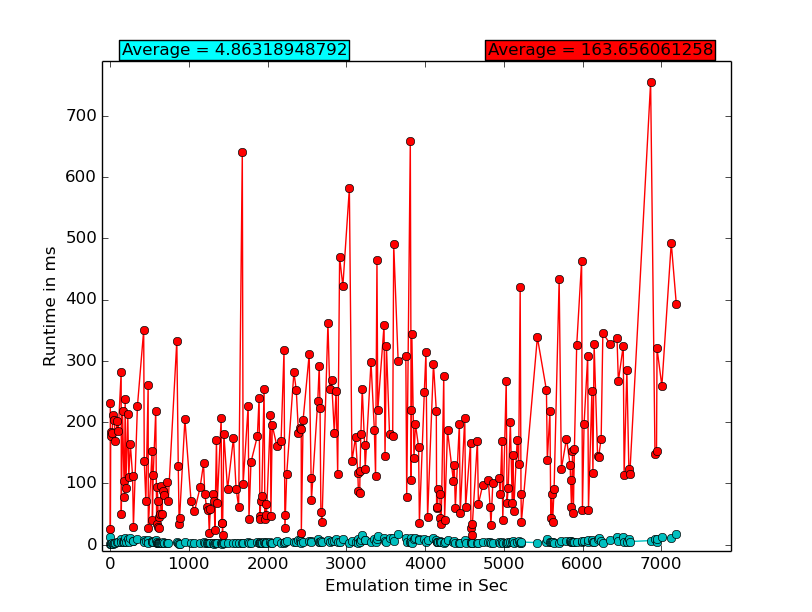
\includegraphics[width=0.48\textwidth]{36ring20genruntime.png}
			\label{fig:ts4runtime}
		}
	\end{center}
\end{figure}

Similar to other scenarios, Figure \ref{fig:ts4runtime} has two statistics: the plotting of $t_{ar}$ against $t_e$ is in cyan and $t_{rr}$ against $t_e$ is in red. Average $t_{ar}$ is around 4.86 ms and the average $t_{rr}$ is around 163.65 ms. Similar to scenario 3, the average $t_{rr}$ is low because of generic flow type. Like other generic scenarios, here the algorithm execution also happened very frequently.

\subsection{Test Scenario 5}
This scenario was also executed in MaxiNet platform, the load level scale was set to 0.02, mesh topology was used and the type of flow generated for the scenario is CoMP. Figure \ref{fig:ts5timediff} shows the plotting of $t_d$ against $t_e$. Both positive and negative $t_d$ of +11.51 to -3.87 seconds was observed in this scenario. Here, $t_d$ has bigger range since it is a CoMP scenario; when the load is higher, the testbed has to start many iperf instances and configure many traffic control objects which is why more system time passed while the $t_e$ does not move that much. In another case, while load level scale is low (0.02), then the emulation has to add very few flow in the system because of that $t_e$ move ahead of $t_s$.

\begin{figure}[H]
	\begin{center}
		\subfloat[Emulation time vs time difference]{
			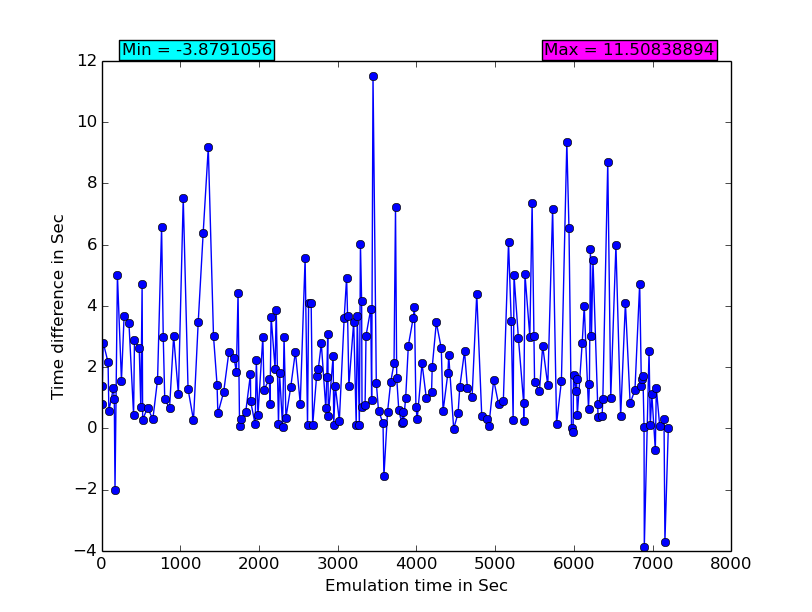
\includegraphics[width=0.48\textwidth]{36mesh02comptimediff.png}
			\label{fig:ts5timediff}
		}
		\subfloat[Emulation time vs runtime]{
			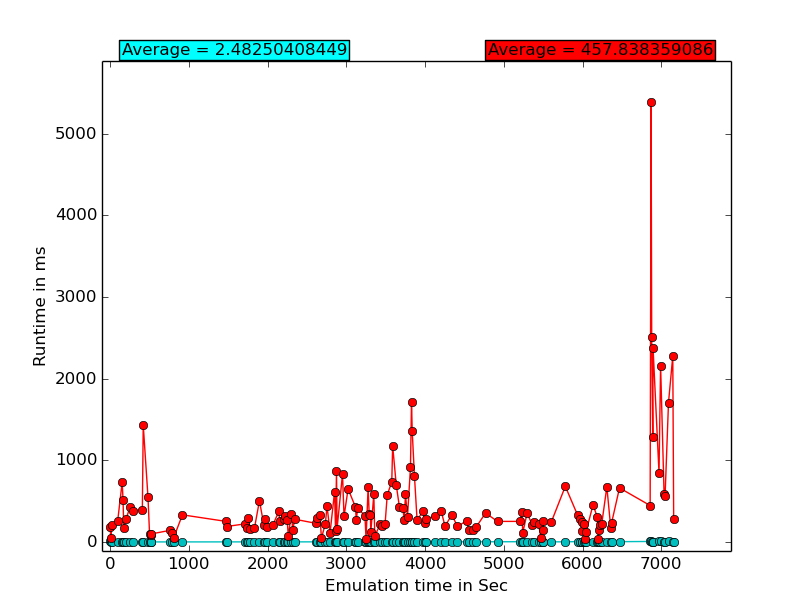
\includegraphics[width=0.48\textwidth]{36mesh02compruntime.png}
			\label{fig:ts5runtime}
		}
	\end{center}
\end{figure}

Similar to other scenarios, Figure \ref{fig:ts5runtime} has two statistics: the plotting of $t_{ar}$ against $t_e$ is in cyan and $t_{rr}$ against $t_e$ is in red. Average $t_{ar}$ is around 2.48 ms and the average $t_{rr}$ is around 457.83 ms. The average $t_{rr}$ is higher because for CoMP flow types, numerous traffic control objects are usually need to be added and for a single DFG, multiple traffic flow generation has to be started. Like other CoMP scenarios, here I observed bigger gaps between the dots, which means less number of algorithm execution happened. I observed a big spike for $t_{rr}$ at the end, which happened because at that algorithm execution, 2 LCA were removed at a time due to low load situation. This means there were many changes in the node to LCA assignment so there are many routing entry needed to be added and deleted in the underlying network. Additionally, there are many DFG which were reassigned, therefore many iperf instances that need to be started.For this reason, the emulation took a lot of time to process those tasks and $t_{rr}$ rose to 5,382 ms.

\subsection{Test Scenario 6}
This scenario was also executed in MaxiNet platform, the load level scale was set to 0.02, a ring topology was used and the type of flow generated for the scenario is CoMP. Figure \ref{fig:ts6timediff} shows the plotting of $t_d$ against $t_e$. Both positive and negative $t_d$ of +13.33 to -0.34 seconds was observed in this scenario. Similar to scenario 5, the load scale is low and flow type is CoMP so a higher range of $t_d$ has been observed in this case.

\begin{figure}[H]
	\begin{center}
		\subfloat[Emulation time vs time difference]{
			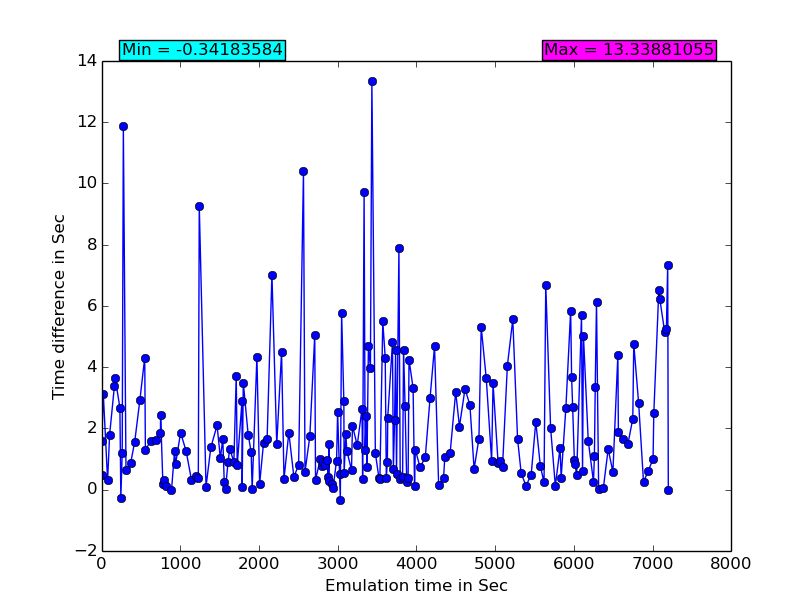
\includegraphics[width=0.48\textwidth]{36ring02comptimediff.png}
			\label{fig:ts6timediff}
		}
		\subfloat[Emulation time vs runtime]{
			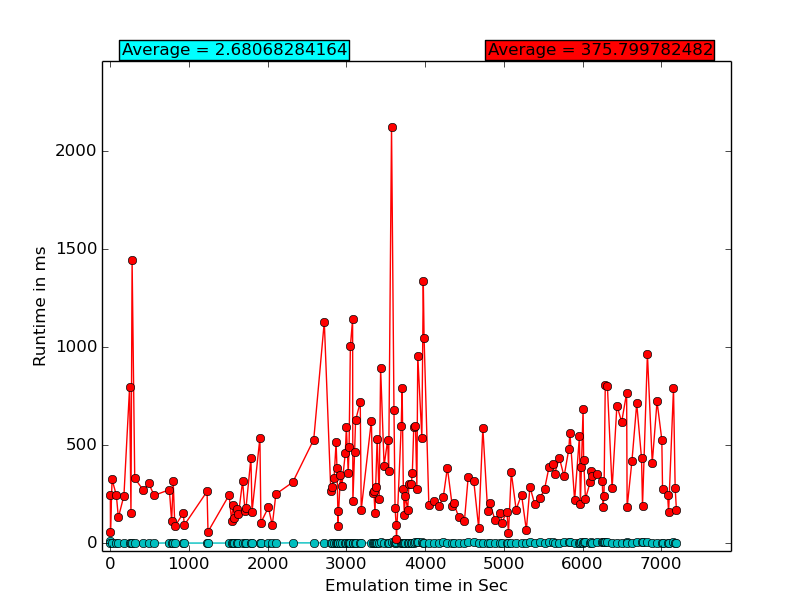
\includegraphics[width=0.48\textwidth]{36ring02compruntime.png}
			\label{fig:ts6runtime}
		}
	\end{center}
\end{figure}

Similar to other scenarios, Figure \ref{fig:ts6runtime} has two statistics: the plotting of $t_{ar}$ against $t_e$ is in cyan and $t_{rr}$ against $t_e$ is in red. Average $t_{ar}$ is around 2.68 ms and the average $t_{rr}$ is around 375.79 ms. Similar to scenario 5, average $t_{rr}$ is high because of the CoMP flow type, and bigger gaps between algorithm run has been observed here as well. 

Usually, in the generic scenario, algorithm runs happen very frequently which means many reassignments happen and which is why there are many fluctuating spikes seen in $t_{rr}$ plotting. Whereas in the case of CoMP scenario, the number of algorithm run was lesser which is why bigger gaps between dots have been observed in $t_{rr}$ plotting. Even though there are very few long spikes in CoMP scenario, the average $t_{rr}$ is very high which means for CoMP scenario there are many traffic control objects to configure and many iperf instances to start after the algorithm run. Another important observation in CoMP scenario is a high range of $t_d$ due to the lesser number of DFG to be added in the system, though the number of traffic control objects to configure and the number of iperf instances to be run is higher which caused higher $t_d$ range. A common pattern is observed across all scenarios, all $t_{rr}$ plotting followed the load level curve specified in Figure \ref{fig:24loadlevel}. Initially, the load is high in the system so $t_{rr}$ is high; it goes down to lowest around 900 seconds then it starts increasing and reach high at around 3,500 seconds and again start decreasing and goes down to lowest around 4,500 seconds and reach high again at around 7,000 seconds.

\section{Comparison with Simulation}\label{sec:cws}
I did not modify the actual FlexFCAPF algorithm for emulation. The algorithm was executed in simulation and the evaluation results of the simulation are presented in \cite{7343600}. I mainly focused on evaluating emulation aspects which were not possible in the simulation. Virtual network elements and hosts are created in the emulation testbed and real application is running on them (ipref, Wireshark, socat, etc.). Actual OpenFlow protocol is used to communicate between the SDN controller and the network elements. The real forwarding entries are populated in the network elements and tested traffic is following the exact path as specified. A real data processing capability is implemented, real traffic is generated and transmitted between hosts, and verified that the traffic bandwidth and duration can be controlled as desired. Finally, the emulation evaluation scenarios are executed in real time so the algorithm performance is proven in a more realistic environment.
\begin{figure}[H]
	\begin{center}
		\subfloat[Simulation time vs number of LCA used]{
			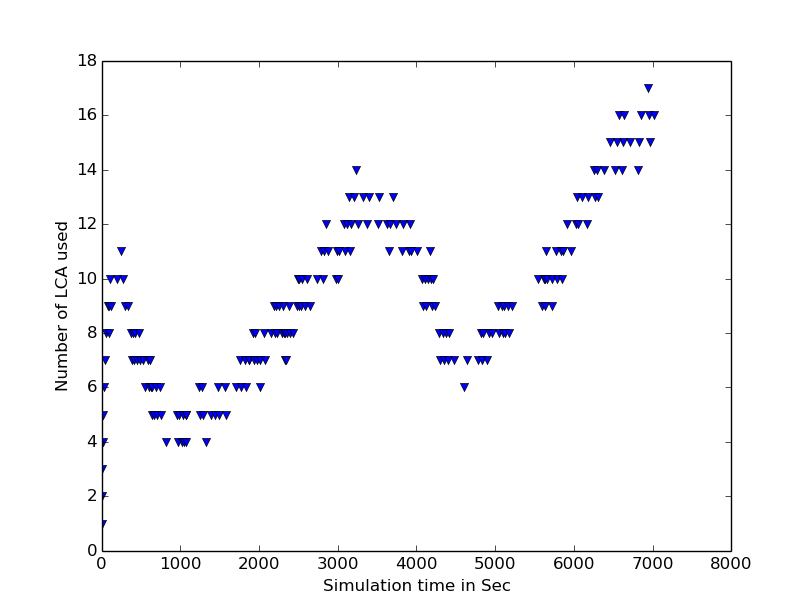
\includegraphics[width=0.48\textwidth]{sim-lcaused.png}
			\label{fig:simlca}
		}
		\subfloat[Emulation time vs number of LCA used]{
			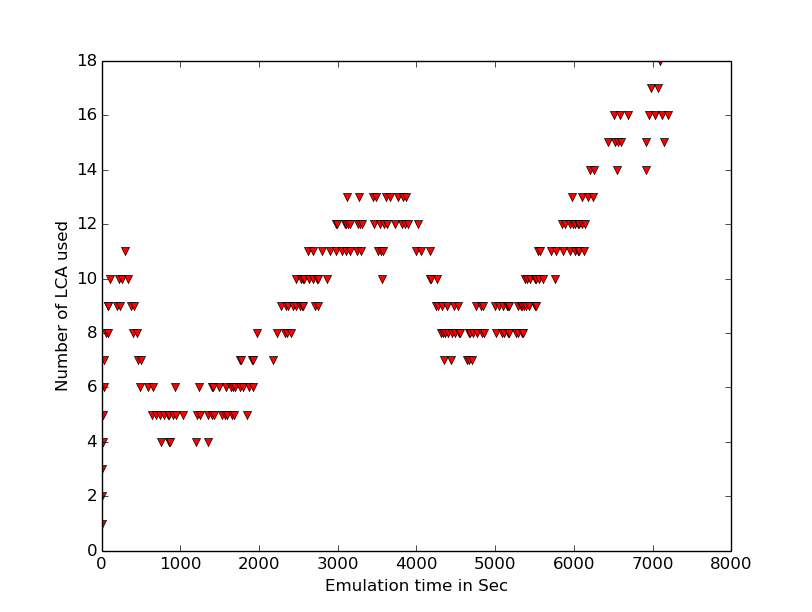
\includegraphics[width=0.48\textwidth]{emu-lcaused.png}
			\label{fig:emulca}
		}
	\end{center}
\end{figure}

I executed a scenario to show that the outcome of the algorithm is independent of the simulation or emulation. Figure \ref{fig:simlca} and \ref{fig:emulca} show the number of LCA used in simulation and emulation execution, respectively. Both simulation and emulation are executed for 7,200 seconds using same topology description (mesh) with 36 nodes and generic type DFG are added during the execution. I observed similar number of LCA used in both cases and LCAs are adjusted in similar pattern during the complete execution.
